\begin{name}
	{Nhóm \LaTeX\ PT THỦ ĐÔ}
	{ĐỀ THI KHẢO SÁT CHẤT LƯỢNG HỌC KỲ II}
\end{name}

\Opensolutionfile{ansbook}[ans/ansb\currfilebase]

%======== PHẦN I. TRẮC NGHIỆM (NHIỀU PHƯƠNG ÁN) ========

\caulc
\Opensolutionfile{ans}[ans/ans\currfilebase-Phan-I]

%Câu 1 (TN)
\begin{ex}%%[2D1H1-1]
	Cho hàm số $y=\dfrac{2\,024x+2023}{x+1}$. Khẳng định nào sau đây là đúng?
	\choice
	{\True Hàm số đồng biến trên mỗi khoảng $(-\infty;-1)$ và $(-1;+\infty)$}
	{Hàm số nghịch biến trên mỗi khoảng $(-\infty;-1)$ và $(-1;+\infty)$}
	{Hàm số đồng biến trên mỗi khoảng $(-\infty;-1)$ và $(1;+\infty)$, nghịch biến trên $(-1 ; 1)$}
	{Hàm số đồng biến trên $\mathbb{R}$}
	\loigiai{
		Tập xác định của hàm số $\mathscr{D}=\mathbb{R}\setminus\{-1\}$.\\ 
		Ta có $y'=\dfrac{1}{(x+1)^2}>0$, $\forall x\in\mathscr{D}$.\\
		Do đó, hàm số đồng biến trên mỗi khoảng $(-\infty;-1)$ và $(-1;+\infty)$.}
\end{ex}

%Câu 2 (TN)
\begin{ex}%%[2D1H1-2]
	Cho hàm số $y=f(x)$ có bảng biến thiên như hình vẽ
	\begin{center}
		
\begin{tikzpicture}
			\tkzTabInit[nocadre=true, lgt=1.2, espcl=2.5, deltacl=0.5]
			{$x$/ 0.7,$f'(x) $/0.7,$f(x)$/2}
			{$-\infty$,$-1$,$0$,$1$,$+\infty$}
			\tkzTabLine{,-,0,+,0,-,0,+,}
			\tkzTabVar{+/$+\infty$,-/$-3$, +/$-2$,-/$-3$, +/$+\infty$} %dấu mũi tên, + trên, - dưới
		\end{tikzpicture}
	\end{center}
	Hàm số đã cho đồng biến trên khoảng nào dưới đây?
	\choice
	{\True $(1;+\infty)$}
	{$(0;+\infty)$}
	{$(-\infty;-1)$}
	{$(-1;1)$}
	\loigiai{
		Từ bảng biến thiên ta có hàm số đã cho đồng biến trên $(-1;0)$ và $(1;+\infty)$.
	}
\end{ex}

%Câu 3 (TN)
\begin{ex}%%[2D4N2-1]
	Nếu $\displaystyle\int\limits_1^2 f(x)\mathrm{\,d}x=2$ và $\displaystyle\int\limits_0^2  f(x)\mathrm{\,d}x=4$ thì $\displaystyle\int\limits_0^1 f(x)\mathrm{\,d}x$ bằng
	\choice
	{$6$}
	{\True $2$}
	{$8$}
	{$-2$}
	\loigiai{
		Ta có $\displaystyle\int\limits_0^1 f(x)\mathrm{\,d}x=\displaystyle\int\limits_0^2  f(x)\mathrm{\,d}x-\displaystyle\int\limits_1^2 f(x)\mathrm{\,d}x=4-2=2$.
	}
\end{ex}

%Câu 4 (TN)
\begin{ex}%%[2D4H2-4]
	Tìm hàm số $f(x)$ biết $\displaystyle\int f(x)\mathrm{\,d}x=\dfrac{x^2}{2}+\mathrm{e}^x+C$.
	\choice
	{$f(x)=\dfrac{x}{2}+\mathrm{e}^x$}
	{\True $f(x)=x+\mathrm{e}^x$}
	{$f(x)=\dfrac{x^3}{3}+\mathrm{e}^x$}
	{$f(x)=\dfrac{x^3}{6}+\mathrm{e}^x$}
	\loigiai{
		Ta có $f(x)=\left(\dfrac{x^2}{2}+\mathrm{e}^x+C\right)'=x+\mathrm{e}^x$.
	}
\end{ex}

%Câu 5 (TN)
\begin{ex}%%[1H8H7-4]
	Cho khối chóp có diện tích đáy $24$\,cm$^2$ và chiều cao $30$\,cm. Thể tích của khối chóp bằng
	\choice
	{\True $240$\,cm$^3$}
	{$220$\,cm$^3$}
	{$280$\,cm$^3$}
	{$260$\,cm$^3$}
	\loigiai{
		Ta có thể tích của khối chóp đã cho là $V=\dfrac{1}{3}B\cdot h=\dfrac{1}{3}\cdot 24\cdot 30=240$\,cm$^3$.
	}
\end{ex}

%Câu 6 (TN)
\begin{ex}[BỎ]
	Trên mặt phẳng tọa độ $Oxy$, điểm biểu diễn số phức $z=-3+2i$ là
	\choice
	{$M(3;2)$}
	{$N(2;3)$}
	{$P(2;-3)$}
	{\True $Q(-3;2)$}
	\loigiai{
		Trên mặt phẳng tọa độ $Oxy$, điểm biểu diễn số phức $z=-3+2i$ là $Q(-3;2)$.
	}
\end{ex}


%Câu 7 (TN)
\begin{ex}%%[2D1H1-1]
	Hàm số $y=\log(3x-2)$ đồng biến trên khoảng nào dưới đây?
	\choice
	{$(0;+\infty)$}
	{\True $(1;2)$}
	{$\left(-\infty;\dfrac{2}{3}\right)$}
	{$\mathbb{R}$}
	\loigiai{
		Tập xác định của hàm số $y=\log(3x-2)$  là $\mathscr{D}=\left(\dfrac{2}{3};+\infty\right)$.\\
		Hàm số $y=\log(3x-2)$ đồng biến trên $\mathscr{D}$ (vì có cơ số $a=10>1$) nên hàm số đã cho đồng biến trên $(1;2)$.
	}
\end{ex}

%Câu 8 (TN)
\begin{ex}%%[1D6H4-3]
	Số nghiệm nguyên dương của bất phương trình $\log _{\tfrac{1}{2}}(4x-9)>\log _{\tfrac{1}{2}}(x+10)$ là
	\choice
	{$5$}
	{Vô số}
	{\True $4$}
	{$6$}
	\loigiai{
		Điều kiện $\heva{&4x-9>0\\&x+10>0}\Leftrightarrow x>\dfrac{9}{4}$.\\
		Với điều kiện $x>\dfrac{9}{4}$, ta có bất phương trình đã cho tương đương với 
		\[4x-9<x+10\Leftrightarrow x<\dfrac{19}{3}.\]
		So với điều kiện, ta có nghiệm của bất phương trình là $\dfrac{9}{4}<x<\dfrac{19}{3}$.\\
		Vậy bất phương trình có bốn nghiệm nguyên dương là $\{3;4;5;6\}$.
	}
\end{ex}

%Câu 9 (TN)
\begin{ex}%%[2H5H1-3]
	Trong không gian $Oxyz$, mặt phẳng $(P)$ đi qua hai điểm $A(2;-1;4)$, $B(3;2;-1)$ và vuông góc với mặt phẳng $(Q)\colon x+y+2z-1=0$ có phương trình là
	\choice
	{$-11x-7y+2z+7=0$}
	{\True $11x-7y-2z-21=0$}
	{$-11x+7y-2z+49=0$}
	{$11x+7y+2z+23=0$}
	\loigiai{
		Ta có $\overrightarrow{AB}=(1;3;-5)$.\\
		Mặt phẳng $(Q)$ có một vectơ pháp tuyến là $\overrightarrow{n}_Q=(1;1;2)$.\\
		Mặt phẳng $(P)$ chứa $AB$ và vuông góc mặt phẳng $(Q)$ nên nhận $\overrightarrow{n}=\left[\overrightarrow{AB},\overrightarrow{n}_Q\right]=(11;-7;-2)$ làm một vectơ pháp tuyến.\\
		Khi đó, mặt phẳng $(P)$ qua $A(2;-1;4)$ và có $\overrightarrow{n}=(11;-7;-2)$ là vectơ pháp tuyến nên có phương trình là
		\[11(x-2)-7(y+1)-2(z-4)=0\Leftrightarrow 11x-7y-2z-21=0.\]
	}
\end{ex}

%Câu 10 (TN)
\begin{ex}%%[2H2H2-2]
	Trong không gian $Oxyz$, cho điểm $A$ thỏa mãn điều kiện $\overrightarrow{AO}=-3\overrightarrow{i}-2\overrightarrow{j}-\overrightarrow{k}$. Tìm tọa độ điểm $A'$ đối xứng với điểm $A$ qua mặt phẳng $(Oxy)$.
	\choice
	{$A'(-3;-2;1)$}
	{$A'(-3;-2;0)$}
	{$A'(3;2;0)$}
	{\True $A'(3;2;-1)$}
	\loigiai{
		Ta có 
		\[\overrightarrow{AO}=-3\overrightarrow{i}-2\overrightarrow{j}-\overrightarrow{k}\Rightarrow \overrightarrow{OA}=3\overrightarrow{i}+2\overrightarrow{j}+\overrightarrow{k}\Rightarrow A(3;2;1).\]
		Do đó, tọa độ điểm đối xứng của $A$ qua mặt phẳng $(Oxy)$ là $A'(3;2;-1)$.
	}
\end{ex}

%Câu 11 (TN)
\begin{ex}%%[2H5H3-1]
	Tìm tất cả các giá trị của tham số $m$ để phương trình $x^2+y^2+z^2+4x-2y+2z+m=0$ là phương trình mặt cầu.
	\choice
	{$m>6$}
	{$m>-6$}
	{$m<-6$}
	{\True $m<6$}
	\loigiai{
		Ta có $x^2+y^2+z^2+4x-2y+2z+m=0$ là phương trình mặt cầu khi và chỉ khi 
		\[(-2)^2+1^2+(-1)^2-m>0 \Leftrightarrow m<6.\]
	}
\end{ex}

%Câu 12 (TN)
\begin{ex}%%[2H5H2-3]
	Trong không gian $Oxyz$, đường thẳng đi qua điểm $M(5;7;1)$ và vuông góc với mặt phẳng $(P)\colon 2x-4y+3z+2=0$ có phương trình là
	\choice
	{$\dfrac{x+2}{5}=\dfrac{y-4}{7}=\dfrac{z+3}{1}$}
	{\True $\dfrac{x-5}{2}=\dfrac{y-7}{-4}=\dfrac{z-1}{3}$}
	{$\dfrac{x-2}{5}=\dfrac{y+4}{7}=\dfrac{z-3}{1}$}
	{$\dfrac{x+5}{2}=\dfrac{y+7}{-4}=\dfrac{z+1}{3}$}
	\loigiai{
		Gọi $d$ là đường thẳng đi qua điểm $M(5;7;1)$ và vuông góc với mặt phẳng \break$(P)\colon 2x-4y+3z+2=0$.\\
		Vì $d \perp (P)$ nên đường thẳng $d$ có một vectơ chỉ phương là $\overrightarrow{u}_d=\overrightarrow{n}_P=(2;-4;3)$.\\
		Khi đó, $d$ qua $M(5;7;1)$ và nhận $\overrightarrow{u}_d=(2;-4;3)$ là một vectơ chỉ phương nên có phương trình chính tắc là
		\[\dfrac{x-5}{2}=\dfrac{y-7}{-4}=\dfrac{z-1}{3}.\]
	}
\end{ex}

%Câu 13 (TN)
\begin{ex}%%[1H8N7-4]
	Thể tích khối lăng trụ có diện tích đáy $B$ và có chiều cao $h$ là
	\choice
	{\True $Bh$}
	{$3Bh$}
	{$\dfrac{4}{3}Bh$}
	{$\dfrac{1}{3}Bh$}
	\loigiai{
		Công thức tính thể tích của khối lăng trụ có diện tích đáy $B$ và có chiều cao $h$ là $V=Bh$.
	}
\end{ex}

%Câu 14 (TN)
\begin{ex}%%[1D7H2-1]
	Đạo hàm của hàm số $y=2\,024^x$ là
	\choice
	{$y'=\dfrac{2\,024^x}{\ln 2\,024}$}
	{$y'=2\,024\cdot 2\,023^x$}
	{\True $y'=2\,024^x\cdot\ln 2\,024$}
	{$y'=2\,024^x$}
	\loigiai{
		Hàm số $y=2\,024^x$ có đạo hàm là $y'=2\,024^x\cdot\ln 2\,024$.
	}
\end{ex}

%Câu 15 (TN)
\begin{ex}[BỎ]
	Cho số phức $z=1-3i$. Môđun của số phức $(1-i)z$ bằng
	\choice
	{$10$}
	{\True $2\sqrt{5}$}
	{$20$}
	{$5 \sqrt{2}$}
	\loigiai{
		Ta có $\left|(1-i)z\right|=\left|(1-i)(1-3i)\right|=\left|1-i\right|\cdot \left|1-3i\right|=\sqrt{2}\cdot\sqrt{10}=2\sqrt{5}$.
	}
\end{ex}

%Câu 16 (TN)
\begin{ex}%%[1H8H7-4]
	\immini[thm]{Cho khối lăng trụ đứng $ABC.A'B'C'$ có đáy là tam giác đều cạnh $a$, $AA'=2a$ (tham khảo hình vẽ bên). Thể tích của khối lăng trụ đã cho bằng
		\choice[2]
		{$\sqrt{3} a^3$}
		{$\dfrac{\sqrt{3} a^3}{6}$}
		{\True $\dfrac{\sqrt{3} a^3}{2}$}
		{$\dfrac{\sqrt{3} a^3}{3}$}}{
		
		\begin{tikzpicture}[font=\footnotesize,line join=round, line cap=round, >=stealth,scale=1] 
			\def\a{2.5}
			\def\h{2.75}
			\path 	(0:0) coordinate (A)
			++(0:\a) coordinate (C)
			++(-140:\a*0.6) coordinate (B)
			($(A)+(90:\h)$) coordinate (A')
			($(B)+(90:\h)$) coordinate (B')
			($(C)+(90:\h)$) coordinate (C');
			\draw[dashed] 	(A)--(C);
			\draw	(C)--(C') 	(B)--(B')	(A)--(A') (A)--(B)--(C) (A')--(B')--(C')--cycle;
			\foreach \x/\pos in {A/180,B/-60,C/0,A'/180,B'/-30,C'/0} \fill (\x) circle(1pt) node[{shift=(\pos:0.25)}]{$\x$}; 
	\end{tikzpicture}}
	\loigiai{
		Ta có $\triangle ABC$ là tam giác đều cạnh $a$ nên $S_{\triangle ABC}=\dfrac{\sqrt{3}a^2}{4}$.\\
		Vậy thể tích khối lăng trụ đã cho bằng $V=S_{\triangle ABC}\cdot AA'=\dfrac{\sqrt{3}a^2}{4}\cdot2a=\dfrac{\sqrt{3}a^3}{2}$.
	}
\end{ex}

%Câu 17 (TN)
\begin{ex}[BỎ]
	Cho hình nón có bán kính đáy $r=2$ và độ dài đường sinh $\ell=7$. Diện tích xung quanh của hình nón đã cho bằng
	\choice
	{$28\pi$}
	{\True $14\pi$}
	{$\dfrac{14\pi}{3}$}
	{$\dfrac{98\pi}{3}$}
	\loigiai{
		Ta có diện tích xung quanh của hình nón $S_\text{xq}=\pi\cdot r\cdot \ell=\pi\cdot2\cdot7=14\pi$.}
\end{ex}

%Câu 18 (TN)
\begin{ex}%%[2D4H3-3]
	Thể tích của khối tròn xoay tạo thành khi quay hình phẳng giới hạn bởi đồ thị hàm số $y=x^2-2x$, trục hoành, trục tung và đường thẳng $x=1$ quanh trục hoành bằng
	\choice
	{\True $\dfrac{8 \pi}{15}$}
	{$\dfrac{16 \pi}{15}$}
	{$\dfrac{4 \pi}{3}$}
	{$\dfrac{2 \pi}{3}$}
	\loigiai{
		Thể tích khối tròn xoay khi quay hình phẳng giới hạn bởi $\heva{&y=x^2-2x\\&y=0\\&x=0,\ x=1}$ quanh trục hoành là \[V=\pi\displaystyle\int\limits_0^1\left(x^2-2x\right)^2\mathrm{d}x=\dfrac{8\pi}{15}.\]
	}
\end{ex}

%Câu 19 (TN)
\begin{ex}%%[2D4H1-2]
	Tìm họ các nguyên hàm $F(x)$ của hàm số $f(x)=\dfrac{x+3}{x+1}$.
	\choice
	{$F(x)=x+\ln|x+1|+C$}
	{$F(x)=x-\ln|x+1|+C$}
	{$F(x)=x-3\ln|x+1|+C$}
	{\True $F(x)=x+2\ln|x+1|+C$}
	\loigiai{
		Ta có $f(x)=\dfrac{x+3}{x+1}=1+\dfrac{2}{x+1}$.\\
		Do đó $F(x)=\displaystyle\int f(x)\mathrm{\,d}x=\displaystyle\int \left(1+\dfrac{2}{x+1}\right)\mathrm{d}x=x+2\ln|x+1|+C$.
	}
\end{ex}

%Câu 20 (TN)
\begin{ex}%%[1D6N2-2]
	Đặt $P=\ln(9\mathrm{e})$. Khẳng định nào dưới đây đúng?
	\choice
	{$P=3\ln3+1$}
	{$P=3\ln3$}
	{$P=9\mathrm{e}$}
	{\True $P=2\ln3+1$}
	\loigiai{
		Ta có $P=\ln(9\mathrm{e})=\ln9+\ln\mathrm{e}=2\ln3+1$.
	}
\end{ex}

%Câu 21 (TN)
\begin{ex}[BỎ]
	Biết phương trình $z^2-mz+n=0$ $(m, n \in \mathbb{R})$ có một nghiệm là $z=3+i$. Tính $m-n$.
	\choice
	{$16$}
	{$-16$}
	{$4$}
	{\True  $-4$ }
	\loigiai{
		Phương trình $z^2-mz+n=0$ có một nghiệm là $z_1=3+i$ nên phương trình đã cho có nghiệm còn lại là $z_2=3-i$.\\
		Theo hệ thức Viète, ta có $\heva{&m=z_1+z_2=6\\&n=z_1\cdot z_2=10.}$\\
		Suy ra $m-n=6-10=-4$.
	}
\end{ex}

%Câu 22 (TN)
\begin{ex}%%[2H5N1-5]
	Trong không gian $Oxyz$, cho mặt phẳng $(P)\colon 2x-y+2z-4=0$. Khoảng cách từ điểm $M(3;1;-2)$ đến mặt phẳng $(P)$ bằng
	\choice
	{$\dfrac{1}{3}$}
	{\True $1$}
	{$2$}
	{$3$}
	\loigiai{
		Ta có $\mathrm{d}\big(M,(P)\big)=\dfrac{|2\cdot 3-1+2\cdot (-2)-4|}{\sqrt{2^2+(-1)^2+2^2}}=1$.
	}
\end{ex}

%Câu 23 (TN)
\begin{ex}%%[2D1H5-4]
	\immini[thm]{Cho hàm số bậc bốn $y=f(x)$ có đồ thị như hình vẽ bên. Số nghiệm của phương trình $f(x)=2$ là
		\choice[2]
		{$3$}
		{\True $4$}
		{$1$}
		{$2$}
	}
	{
		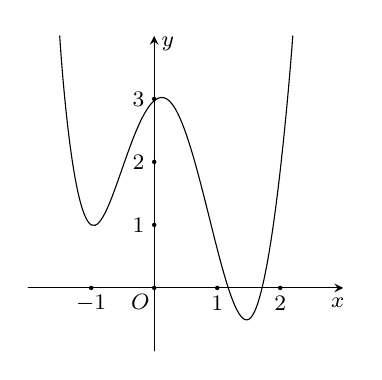
\begin{tikzpicture}[font=\footnotesize,line join=round, line cap=round, >=stealth,scale=0.8] 
			\def \xmin{-2}\def \xmax{3}\def \ymin{-1}\def \ymax{4} 
			\draw[->] (\xmin,0)--(\xmax,0) node[shift=(-110:0.2)] {$x$};
			\draw[->] (0,\ymin)--(0,\ymax) node[shift=(-30:0.2)] {$y$};
			\fill (0,0) circle(1pt) node[shift=(-135:0.25)]{$O$}; 
			\clip (\xmin,\ymin) rectangle (\xmax,\ymax); 
			\draw[smooth,samples=100,domain=\xmin:\xmax] plot[smooth,tension=0.7] coordinates{(-1.5,4) (-1,1) (0.2,3) (1.5,-0.5) (2.2,4)};
			\foreach \x in {-1,1,2} \fill (\x,0) circle(1pt) node[{shift=(-90:0.2)}]{$\x$}; 
			\foreach \y in {1,2,3} \fill (0,\y) circle(1pt) node[left]{$\y$}; 
		\end{tikzpicture}
	}
	\loigiai{
		Phương trình $f(x)=2$ là phương trình hoành độ giao điểm của đồ thị hàm số $y=f(x)$ và đường thẳng $y=2$.\\
		\begin{center}
			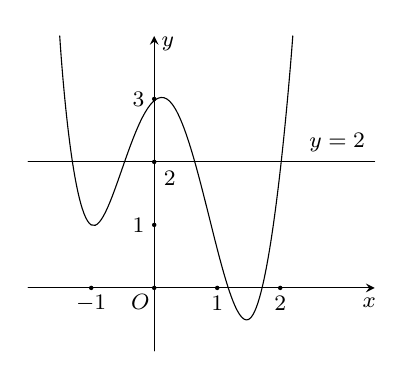
\begin{tikzpicture}[font=\footnotesize,line join=round, line cap=round, >=stealth,scale=0.8] 
				\def \xmin{-2}\def \xmax{3.5}\def \ymin{-1}\def \ymax{4} 
				\draw[->] (\xmin,0)--(\xmax,0) node[shift=(-110:0.2)] {$x$};
				\draw[->] (0,\ymin)--(0,\ymax) node[shift=(-30:0.2)] {$y$};
				\fill (0,0) circle(1pt) node[shift=(-135:0.25)]{$O$}; 
				\draw(\xmin,2)--(\xmax,2) node[above left]{$y=2$};
				\clip (\xmin,\ymin) rectangle (\xmax,\ymax); 
				\draw[smooth,samples=100,domain=\xmin:\xmax] plot[smooth,tension=0.7] coordinates{(-1.5,4) (-1,1) (0.2,3) (1.5,-0.5) (2.2,4)};
				\foreach \x in {-1,1,2} \fill (\x,0) circle(1pt) node[{shift=(-90:0.2)}]{$\x$}; 
				\foreach \y in {1,3} \fill (0,\y) circle(1pt) node[left]{$\y$}; 
				\foreach \y in {2} \fill (0,\y) circle(1pt) node[below right]{$\y$}; 
			\end{tikzpicture}
		\end{center}
		Vẽ thêm đường thẳng $y=2$ và đồ thị hàm số $y=f(x)$ trên cùng hệ trục tọa độ, ta thấy hai đường cắt nhau tại $4$ điểm phân biệt.\\
		Suy ra, phương trình $f(x)=2$ có $4$ nghiệm phân biệt.
	}
\end{ex}

%Câu 24 (TN)
\begin{ex}%%[2D1H3-1]
	Giá trị lớn nhất của hàm số $f(x)=x^3-3x^2+2$ trên đoạn $[1;3]$ bằng
	\choice
	{$3$}
	{$-2$}
	{\True $2$}
	{$0$ }
	\loigiai{
		Ta có $f'(x)=3x^2-6x$. \\
		Phương trình $f'(x)=0\Leftrightarrow \hoac{&x=0\not \in [1;3]\\&x=2 \in [1;3].}$\\
		Ta có $f(1)=0$; $f(2)=-2$; $f(3)=2$.\\
		Suy ra $\max \limits_{[1;3]} f(x)=2$ khi $x=3$.
	}
\end{ex}

%Câu 25 (TN)
\begin{ex}%%[2D1H2-2]
	Cho hàm số $y=f(x)$ có bảng biến thiên như sau:
	\begin{center}
		
\begin{tikzpicture}
			\tkzTabInit[nocadre=true, lgt=1 , espcl=3, deltacl=0.5] 
			{$x$ / 0.7,$y'$ /.7,$y$/2}
			{$-\infty$,$1$,$3$,$+\infty$}
			\tkzTabLine{,+,0,-,0,+,}
			\tkzTabVar{-/$-\infty$,+/$2$,-/$-2$,+/$+\infty$}
		\end{tikzpicture}
	\end{center}
	Hàm số đã cho đạt cực đại tại
	\choice
	{$x=3$}
	{\True $x=1$}
	{$x=-2$}
	{$x=2$}
	\loigiai{
		Từ bảng biến thiên, ta thấy hàm số đã cho đạt cực đại tại $x=1$.
	}
\end{ex}

%Câu 26 (TN)
\begin{ex}%%[1D6H4-2]
	Phương trình $3^{x-2}=27$ có nghiệm là
	\choice
	{$x=1$}
	{$x=3$}
	{\True $x=5$}
	{$x=-5$}
	\loigiai{
		Ta có $3^{x-2}=27\Leftrightarrow 3^{x-2}=3^3\Leftrightarrow x-2=3\Leftrightarrow x=5$.\\
		Vậy phương trình đã cho có nghiệm là $x=5$.
	}
\end{ex}

%Câu 27 (TN)
\begin{ex}%%[2H5N2-2]
	Trong không gian $Oxyz$, cho đường thẳng $d\colon \dfrac{x-3}{2}=\dfrac{y-4}{-5}=\dfrac{z+1}{3}$. Vectơ nào sau đây là một vectơ chỉ phương của $d$?
	\choice
	{\True $\overrightarrow{w}=(2;-5; 3)$}
	{$\overrightarrow{r}=(2; 5; 3)$}
	{$\overrightarrow{v}=(3; 4;-1)$}
	{$\overrightarrow{u}=(3; 4; 1)$}
	\loigiai{
		Một vectơ chỉ phương của đường thẳng $d$ là $\overrightarrow{w}=(2;-5; 3)$.
	}
\end{ex}

%Câu 28 (TN)
\begin{ex}[BỎ]
	Tính tích phân $I=\displaystyle \int\limits_0^{\tfrac{\pi}{2}} \cos^{7}x\cdot \sin x \mathrm{\,d}x$ bằng cách đặt $t=\cos x$, khẳng định nào dưới đây đúng?
	\choice
	{\True $I=\displaystyle\int\limits_0^1{t^7}\mathrm{\,d}t$}
	{$I=-\displaystyle\int\limits_0^1{t^7}\mathrm{\,d}t$}
	{$I=\displaystyle\int\limits_0^{\tfrac{\pi}{2}}{t^7}\mathrm{\,d}t$}
	{$I=-\displaystyle \int\limits_0^{\tfrac{\pi}{2}}{t^7}\mathrm{\,d}t$}
	\loigiai{
		Đặt $t=\cos x\Rightarrow \mathrm{\, d} t=-\sin x \mathrm{\, d} x$.\\
		Đổi cận $x=0\Rightarrow t=1$; $x=\dfrac{\pi }{2}\Rightarrow t=0$.\\
		$\Rightarrow I=\displaystyle\int\limits_0^{\tfrac{\pi}{2}} \cos^7 x\cdot \sin x \mathrm{\,d}x
		=-\displaystyle\int\limits_1^0 {t^7}\mathrm{\,d}t
		=\displaystyle\int\limits_0^1 {t^7}\mathrm{\,d}t$.
	}
\end{ex}

%Câu 29 (TN)
\begin{ex}[BỎ]
	Giả sử $I=\displaystyle\int\limits_1^4(x-1) \ln x \mathrm{\, d} x=a \ln 2-\dfrac{b}{c}$, trong đó $a, b, c$ là các số nguyên dương và $\dfrac{b}{c}$ là phân số tối giản. Tính $S=a+b+c$.
	\choice
	{$S=9$}
	{$S=12$}
	{\True $S=15$}
	{$S=14$}
	\loigiai{
		Đặt $\heva{&u=\ln x\\&\mathrm{\,d} v=(x-1)\mathrm{\,d}x}\Rightarrow \heva{&\mathrm{\,d}u=\dfrac{1}{x}\mathrm{\,d} x\\&v=\dfrac{1}{2}x^2-x.}$\\
		Khi đó, ta có
		\allowdisplaybreaks \begin{align*}
			I&=\left[\left(\dfrac{1}{2}x^2-x\right)\ln x\right]\Big|_1^4 -\displaystyle\int\limits_1^4 \left(\dfrac{1}{2}x-1\right)\mathrm{d}x\\
			&=\left[\left(\dfrac{1}{2}x^2-x\right)\ln x\right]\Big|_1^4 -\left(\dfrac{1}{4}x^2-x\right)\bigg|_1^4\\&=4\ln 4-\dfrac{3}{4}=8\ln 2-\dfrac{3}{4}.
		\end{align*}
		Suy ra $a=8$; $b=3$; $c=4$.\\
		Vậy $S=a+b+c=15$.
	}
\end{ex}

%Câu 30 (TN)
\begin{ex}%%[2D1H4-1]
	Đường tiệm cận đứng của đồ thị hàm số $y=\dfrac{x+2\,023}{x-2\,024}$ là
	\choice
	{\True $x=2\,024$}
	{$y=2\,024$}
	{$x=-2\,023$}
	{$y=1$}
	\loigiai{
		Ta có $\lim\limits_{x\to 2024^+}y=\lim\limits_{x\to 2024^+}\dfrac{x+2\,023}{x-2\,024}=+\infty$.\\
		Đường tiệm cận đứng của đồ thị hàm số $y=\dfrac{x+2\,023}{x-2\,024}$ là đường thẳng $x=2024$.
	}
\end{ex}

%Câu 31 (TN)
\begin{ex}%%[2D1H5-1]
	\immini[thm]{Đồ thị của hàm số nào dưới đây có dạng như đường cong trong hình vẽ bên?
		\choice[2]
		{$y=-x^4+2x^2+2$}
		{$y=x^4-2x^2+2$}
		{\True $y=x^3-x+2$}
		{$y=-x^3+x+2$}}{
		\begin{tikzpicture}[font=\footnotesize,line join=round, line cap=round, >=stealth,scale=0.8] 
			\def \xmin{-2}\def \xmax{2}\def \ymin{-1}\def \ymax{3} 
			\draw[->] (\xmin,0)--(\xmax,0) node[shift=(-110:0.2)] {$x$};
			\draw[->] (0,\ymin)--(0,\ymax) node[shift=(-30:0.2)] {$y$};
			\fill (0,0) circle(1pt) node[shift=(-135:0.25)]{$O$};
			\clip (\xmin,\ymin) rectangle (\xmax,\ymax);
			\draw[smooth,samples=100,domain=\xmin:\xmax] plot(\x,{(\x)^3-(\x)+2}); 
	\end{tikzpicture}}
	\loigiai{
		Đồ thị có dạng như hình vẽ là đồ thị hàm số bậc ba $y=a x^3+bx^2+cx+d$ với $a>0$.\\
		Do đó, phương án thỏa mãn bài toán là $y=x^3-x+2024$.
	}
\end{ex}

%Câu 32 (TN)
\begin{ex}[BỎ]%Câu 32:
	Cho số phức $z=3-4i$. Mệnh đề nào dưới đây \textbf{sai}?
	\choice
	{Môđun của số phức $z$ bằng $5$}
	{Phần thực và phần ảo của $z$ lần lượt là $3$ và $-4$}
	{\True Số phức liên hợp của $z$ là $\dfrac{3}{5}+\dfrac{4}{5}i$}
	{Điểm biểu diễn số phức $z$ trên mặt phẳng tọa độ là $M(3;-4)$}
	\loigiai{
		Số phức liên hợp của $z$ là $\overline{z}=3+4i$.
	}
\end{ex}

%Câu 33 (TN)
\begin{ex}%%[2H2N2-2]%Câu 33:
	Trong không gian $Oxyz$, hình chiếu vuông góc của điểm $M(3;-2; 2)$ trên trục $Oy$ có tọa độ là
	\choice
	{$(0; 0; 2)$}
	{\True $(0;-2; 0)$}
	{$(3; 0; 0)$}
	{$(3; 0; 2)$}
	\loigiai{
		Hình chiếu vuông góc của điểm $M(3;-2; 2)$ trên trục $Oy$ có tọa độ là $(0;-2; 0)$.
	}
\end{ex}

%Câu 34 (TN)
\begin{ex}%%[2D4H3-1]%Câu 34:
	\immini{Cho hàm số bậc ba $y=f(x)$ có đồ thị như hình vẽ bên. Diện tích hình phẳng $S$ giới hạn bởi đồ thị hàm số $y=f(x)$ và trục $Ox$ được tính bởi công thức
		\choice
		{$S=\displaystyle \int\limits_0^2 f(x) \mathrm{\,d}x-\displaystyle\int\limits_{-1}^0 f(x) \mathrm{\,d}x$}
		{\True $S=\displaystyle \int\limits_{-1}^0 f(x) \mathrm{\,d}x-\displaystyle\int\limits_0^2 f(x) \mathrm{\,d}x$}
		{$S=\displaystyle \int\limits_{-1}^2 f(x) \mathrm{\,d}x$}
		{$S=\displaystyle \int\limits_{-1}^2-f(x) \mathrm{\,d}x$}}{
		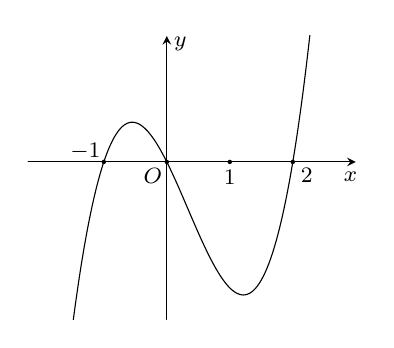
\begin{tikzpicture}[font=\footnotesize,line join=round, line cap=round, >=stealth,scale=0.8] 
			\def \xmin{-2.2}\def \xmax{3}\def \ymin{-2.5}\def \ymax{2} 
			\draw[->] (\xmin,0)--(\xmax,0) node[shift=(-110:0.2)] {$x$};
			\draw[->] (0,\ymin)--(0,\ymax) node[shift=(-30:0.2)] {$y$};
			\fill (0,0) circle(1pt) node[shift=(-135:0.25)]{$O$}
			(-1,0) circle(1pt) node[shift=(150:0.27)]{$-1$}
			(1,0) circle(1pt) node[shift=(-90:0.2)]{$1$}
			(2,0) circle(1pt) node[shift=(-45:0.25)]{$2$}; 
			\clip (\xmin,\ymin) rectangle (\xmax,\ymax);
			\draw[smooth,samples=100,domain=\xmin:\xmax] plot(\x,{(\x+1)*(\x)*(\x-2)}); 
		\end{tikzpicture}
	}
	\loigiai{
		Từ đồ thị hàm số ta thấy diện tích cần tìm là $S=\displaystyle \int\limits_{-1}^0 f(x) \mathrm{\,d}x-\displaystyle\int\limits_0^2 f(x) \mathrm{\,d}x$.
	}
\end{ex}

%Câu 35 (TN)
\begin{ex}[BỎ]%Câu 35:
	Cho số phức $z$ thỏa mãn $z+3 \overline{z}=12+4i$. Số phức nghịch đảo của số phức $z$ là
	\choice
	{$\dfrac{2}{13}-\dfrac{3}{13}i$}
	{$\dfrac{1}{13}-\dfrac{3}{13}i$}
	{$\dfrac{3}{13}-\dfrac{2}{13}i$}
	{\True $\dfrac{3}{13}+\dfrac{2}{13}i$}
	\loigiai{
		Đặt $z=a+bi$ ($a,b\in \mathbb{R}$).\\
		Ta có 
		\allowdisplaybreaks \begin{eqnarray*}
			z+3 \overline{z}=12+4i&\Leftrightarrow& a+bi+3a-3bi=12+4i\\
			& \Leftrightarrow& 4a-2bi=12+4i\\
			&\Leftrightarrow& \heva{&4a=12\\&-2b=4}\Leftrightarrow \heva{&a=3\\&b=-2.}
		\end{eqnarray*}
		Từ đó $z=3-2i\Rightarrow \dfrac{1}{z}=\dfrac{3}{13}+\dfrac{2}{13}i$.
	}
\end{ex}

%Câu 36 (TN)
\begin{ex}[BỎ]
	Gọi $x$, $y$ là các số thực thỏa mãn $(2x-y)i+y(-3-4i)=3+7i$. Giá trị biểu thức $x+y$ bằng
	\choice
	{\True $0$}
	{$2$}
	{$-2$}
	{$-1$}
	\loigiai{
		Ta có 
		\allowdisplaybreaks \begin{eqnarray*}
			&&(2x-y)i+y(-3-4i)=3+7i\\
			&\Leftrightarrow& -3y+(2x-5y)i=3+7i\\
			&\Leftrightarrow& \heva{&-3y=3\\&2x-5y=7}\\
			&\Leftrightarrow& \heva{&y=-1\\&x=1.}
		\end{eqnarray*}
		Vậy $x+y=0$.
	}
\end{ex}

%Câu 37 (TN)
\begin{ex}%%[1D6H1-2]
	Cho $a$ là một số thực dương tùy ý và $a\ne 1$, biểu thức $a^{\tfrac{2}{3}}\sqrt{a}$ bằng
	\choice
	{$a^{\tfrac{6}{7}}$}
	{$a^{\tfrac{5}{7}}$}
	{$a^{\tfrac{4}{3}}$}
	{\True $a^{\tfrac{7}{6}}$}
	\loigiai{
		Ta có $a^{\tfrac{2}{3}}\sqrt{a}=a^{\tfrac{2}{3}+\tfrac{1}{2}}=a^{\tfrac{7}{6}}$.	
	}
\end{ex}

%Câu 38 (TN)
\begin{ex}%%[2H5N3-2]
	Trong không gian $Oxyz$, mặt cầu tâm $I(1;0;0)$ và bán kính bằng $2$ có phương trình là
	\choice
	{$(x-1)^2+y^2+z^2=2$}
	{$(x+1)^2+y^2+z^2=4$}
	{$(x+1)^2+y^2+z^2=2$}
	{\True $(x-1)^2+y^2+z^2=4$}
	\loigiai{
		Mặt cầu tâm $I(1;0;0)$ và bán kính bằng $2$ có phương trình là $(x-1)^2+y^2+z^2=4$.
	}
\end{ex}

%Câu 39 (TN)
\begin{ex}%%[2D4V3-3]
	\immini[thm]{Hình phẳng được tô đậm trong hình vẽ bên được giới hạn bởi đường tròn, đường parabol, trục hoành. Thể tích khối tròn xoay được tạo thành khi quay hình phẳng đã cho quanh trục $Ox$ bằng
		\choice[2]
		{$\left(\dfrac{60\sqrt{2}-40-16\pi}{15}\right)\pi$}
		{$\left(\dfrac{64\sqrt{2}-35-16\pi}{15}\right)\pi$}
		{\True $\left(\dfrac{64\sqrt{2}-36-15\pi}{15}\right)\pi$}
		{$\left(\dfrac{62\sqrt{2}-35-15\pi}{15}\right)\pi$}
	}
	{
		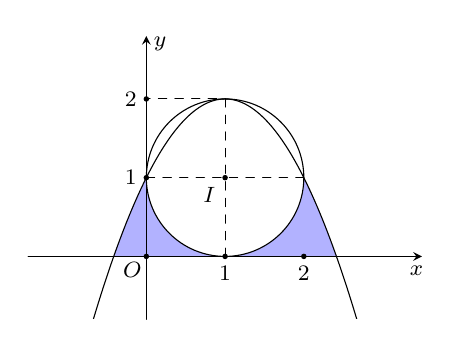
\begin{tikzpicture}[font=\footnotesize,line join=round, line cap=round, >=stealth,scale=1] 
			\def \xmin{-1.5}
			\def \xmax{3.5}
			\def \ymin{-0.8}
			\def \ymax{2.8}
			\pgfmathsetmacro\i{sqrt(2)}
			\fill[blue!30,smooth] 
			(-\i+1,0)--
			plot[domain=-\i+1:\i+1] (\x,{-(\x-1)^2+2})
			--(\i+1,0) --cycle
			;
			\draw[fill=white] (1,1) circle(1);
			%Tự động
			\draw[->] (\xmin,0)--(\xmax,0) node[shift=(-110:0.2)] {$x$};
			\draw[->] (0,\ymin)--(0,\ymax) node[shift=(-30:0.2)] {$y$}; 
			\fill (0,0) circle(1pt) node[shift=(-135:0.25)]{$O$}; 
			%Vẽ các điểm trên 2 hệ trục
			\draw[dashed] (1,0)--(1,2)--(0,2)
			(0,1)--(2,1)
			;
			\fill
			(1,0) circle(1pt) node[below]{$1$}
			(2,0) circle(1pt) node[below]{$2$}
			(0,1) circle(1pt) node[left]{$1$}
			(0,2) circle(1pt) node[left]{$2$}
			(1,1) circle(1pt) node[below left]{$I$}
			;		
			
			%Tự động
			\begin{scope}
				\clip (\xmin+0.01,\ymin+0.01) rectangle (\xmax-0.01,\ymax-0.01);
				\draw[samples=350,domain=\xmin+0.01:\xmax-0.01,smooth,variable=\x] plot (\x,{-(\x-1)^2+2});
			\end{scope}
		\end{tikzpicture}
	}
	\loigiai{
		\begin{center}
			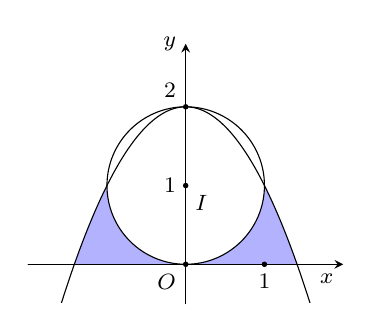
\begin{tikzpicture}[scale=1, font=\footnotesize, line join=round, line cap=round, >=stealth]
				\tikzset{label style/.style={font=\footnotesize}}
				%Nhập giới hạn đồ thị và hàm số cần vẽ
				\def \xmin{-1}
				\def \xmax{3}
				\def \ymin{-0.5}
				\def \ymax{2.8}
				\pgfmathsetmacro\i{sqrt(2)}
				
				\fill[blue!30,smooth] 
				(-\i+1,0)--
				plot[domain=-\i+1:\i+1] (\x,{-(\x-1)^2+2})
				--(\i+1,0) --cycle
				;
				\draw[fill=white] (1,1) circle(1);
				%Tự động
				\draw[->] (\xmin,0)--(\xmax,0) node[below left] {$x$};
				\draw[->] (1,\ymin)--(1,\ymax) node[left] {$y$};
				%\fill (0,0) circle(1pt) node [below right] {$O$};
				%Vẽ các điểm trên 2 hệ trục
				%\draw[dashed,red] (1,0)--(1,2)--(0,2) 		(0,1)--(2,1) 		;
				\fill
				(1,0) circle(1pt) node[below left]{$O$}
				(2,0) circle(1pt) node[below]{$1$}
				(1,1) circle(1pt) node[left]{$1$}
				(1,2) circle(1pt) node[above left]{$2$}
				(1,1) circle(1pt) node[below right]{$I$}
				;		
				
				%Tự động
				\begin{scope}
					\clip (\xmin+0.01,\ymin+0.01) rectangle (\xmax-0.01,\ymax-0.01);
					\draw[samples=350,domain=\xmin+0.01:\xmax-0.01,smooth,variable=\x] plot (\x,{-(\x-1)^2+2});
				\end{scope}
			\end{tikzpicture}
		\end{center}
		Tịnh tiến hệ tọa độ theo vectơ $\overrightarrow{u}=(-1;0)$ thì thể tích khối tròn xoay vẫn không đổi.\\
		Khi đó, đường tròn tâm $I(0;1)$ và bán kính $R=1$ có phương trình $x^2+(y-1)^2=1$, suy ra $y=\pm \sqrt{1-x^2}+1$, và parabol $(P)$ có phương trình $y=-x^2+2$.\\
		Giao điểm của $(P)$ và $Ox$ có hoành độ $x=\pm \sqrt{2}$.\\
		Vì đường tròn và parabol đối xứng qua trục tung nên ta chỉ cần tính thể tích khối tròn xoay ở bên phải trục tung và nhân cho $2$.\\
		Phần tô đậm bên phải trục tung được giới hạn bởi các đường 
		\[x=0,\ x=\sqrt{2},\ y=f(x)=-\sqrt{1-x^2}+1,\ y=g(x)=-x^2+2.\]
		Thể tích $V=\pi \displaystyle\int\limits_0^1 \big[f(x)\big]^2\mathrm{\,d}x+\pi\displaystyle\int\limits_1^{\sqrt{2}} \big[g(x)\big]^2\mathrm{\,d}x=(I_1+I_2)\pi$.
		\begin{itemize}
			\item Tính $I_1
			=\displaystyle\int\limits_0^1 \left(1-\sqrt{1-x^2}\right)^2 \mathrm{\,d}x
			=\displaystyle\int\limits_0^1 \left(2-x^2-2\sqrt{1-x^2}\right)\mathrm{d}x
			=\displaystyle\int\limits_0^1\left(2-x^2\right)\mathrm{d}x-2\displaystyle\int\limits_0^1 \sqrt{1-x^2}\mathrm{\,d}x$.\\
			Đặt $x=\sin t$, $t\in \left(-\dfrac{\pi}{2};\dfrac{\pi}{2}\right)$.\\
			Do đó $\mathrm{\,d}x=\cos t\mathrm{\,d}t$.\\
			Suy ra $2\displaystyle\int\limits_0^1 \sqrt{1-x^2}\mathrm{\,d}x
			=2\displaystyle\int\limits_0^{\tfrac{\pi}{2}} \cos t \cdot \cos t\mathrm{\,d}t
			=\displaystyle\int\limits_0^{\tfrac{\pi}{2}} (1+\cos 2t) \mathrm{\,d}t
			=\left(t+\dfrac{1}{2}\cdot \sin 2t\right)\bigg|_0^{\tfrac{\pi}{2}}=\dfrac{\pi}{2}$.\\
			Vậy $I_1=\dfrac{5}{3}-\dfrac{\pi}{2}$.
			\item Tính $I_2$.\\
			$I_2=\displaystyle\int\limits_1^{\sqrt{2}}\left(-x^2+2\right)^2\mathrm{d}x=\displaystyle\int\limits_1^{\sqrt{2}} \left(x^4-4x^2+4\right)\mathrm{d}x=\left(-\dfrac{x^5}{5}-\dfrac{4x^3}{3}+4x\right)\bigg|_1^{\sqrt{2}}=\dfrac{32\sqrt{2}-43}{15}$.
		\end{itemize}
		Vậy thể tích của khối tròn xoay là \[V'=2V
		=2\pi\left(\dfrac{5}{3}-\dfrac{\pi}{2}+\dfrac{32\sqrt{2}-43}{15}\right)
		=\left(\dfrac{64\sqrt{2}-36-15\pi}{15}\right)\pi.\]
	}
\end{ex}

%Câu 40 (TN)
\begin{ex}[BỎ]
	Có bao nhiêu số phức $z$ thỏa mãn $\left|z-3-6i\right|=2$ và $\left|(1+2i)z-1-12i\right|=3\sqrt{5}$?
	\choice
	{$0$}
	{vô số}
	{$1$}
	{\True $2$}
	\loigiai{
		Gọi $M$ là điểm biểu diễn cho số phức $z$ trong mặt phẳng $Oxy$.
		\begin{itemize}
			\item Từ $\left|z-3-6i\right|=2$, suy ra $M$ thuộc đường tròn tâm $A(3;6)$, bán kính $R_1=2$.
			\item Ta có $\left|(1+2i)z-1-12i\right|=3\sqrt{5}\Leftrightarrow \left|z-(5+2i)\right|=3$.\\ 
			Suy ra $M$ thuộc đường tròn tâm $B(5;2)$, bán kính $R_2=3$.
		\end{itemize}
		Ta có $R_2-R_1<AB=2\sqrt{5}<R_1+R_2$ nên hai đường tròn cắt nhau tại $2$ điểm, tương ứng có $2$ giá trị $z$ thỏa mãn bài toán.
	}
\end{ex}

%Câu 41 (TN)
\begin{ex}[BỎ]
	Cho các số thực $x$, $y$ thỏa mãn
	\[
	\log _2\left(x^2+y^2+2 y\right)+\log _3\left(x^2+y^2\right) \leq \log _2 y+\log _3\left(x^2+y^2+16 y\right) .
	\]
	Tìm giá trị lớn nhất của biểu thức $P=x+2y$.
	\choice
	{\True $2+\sqrt{5}$}
	{$6-\sqrt{5}$}
	{$1+2\sqrt{5}$}
	{$3-\sqrt{5}$}
	\loigiai{
		Điều kiện $y>0$.\\
		Bất phương trình tương đương với
		\allowdisplaybreaks \begin{eqnarray*}
			&&\log _2\left(x^2+y^2+2 y\right)-\log _2 y \leq \log _3\left(x^2+y^2+16 y\right) -\log _3\left(x^2+y^2\right)\\
			&\Leftrightarrow& \log_{2}\left(\dfrac{x^2+y^2}{y}+2\right)\leq \log_{3}\left(1+\dfrac{16y}{x^2+y^2}\right).\quad (1)
		\end{eqnarray*}
		Đặt $t=\dfrac{x^2+y^2}{y}~(t>0)$.\\
		$(1)\Rightarrow \log_{2}(t+2)-\log_{3}\left(1+\dfrac{16}{t}\right) \leq 0$.\\
		Xét hàm số $f(t)=\log_{2}(t+2)-\log_{3}\left(1+\dfrac{16}{t}\right)$.\\
		Ta có $f'(t)=\dfrac{1}{(t+2)\ln2}+\dfrac{16}{\left(t^2+16t\right)\ln3}>0$, $\forall t >0$.\\
		Suy ra hàm số đồng biến trên $(0;+\infty)$.\\
		Bảng biến thiên
		\begin{center}
			\begin{tikzpicture}
				\tkzTabInit[nocadre=true, lgt=1.2, espcl=4, deltacl=0.5]
				{$t$/ 0.7,$f'(t)$/0.6,$f(t)$/2}{$0$,$2$,$+\infty$}
				\tkzTabLine{,+,t,+,}
				\path
				(N13)node[above](1){$-\infty$}
				($(N22)!0.5!(N23)$)node(2){$0$}
				(N32)node[below](3){$+\infty$}
				;
				\foreach \x/\y in {1/2,2/3} \draw[-stealth] (\x)--(\y);
			\end{tikzpicture}
		\end{center}
		Từ bảng biến thiên, suy ra 
		\[f(t)\leq 0 \Leftrightarrow t\leq 2 \Leftrightarrow  \dfrac{x^2+y^2}{y}\leq 2
		\Leftrightarrow x^2+(y-1)^2\leq 1.\]
		Gọi $(C)$ là đường tròn tâm $I(0;1)$, bán kính $R=1$ và $(\Delta)$ là đường thẳng có phương trình $x+2y-P=0$.\\
		Cặp số thực $(x;y)$ tồn tại khi và chỉ khi đường thẳng $\Delta$ và đường tròn $(C)$ có điểm chung.\\
		Do đó, điều kiện thỏa mãn bài toán là 
		\[\mathrm{d}\big(I,(\Delta)\big)\leq R \Leftrightarrow |0+2\cdot 1-P|\leq \sqrt{5} \Leftrightarrow 2-\sqrt{5} \leq P \leq 2+\sqrt{5}.\]
		Vậy $P_{\max}=2+\sqrt{5}$.
	}
\end{ex}

%Câu 42 (TN)
\begin{ex}[BỎ]
	Cho hai số phức $z_1$, $z_2$ thỏa mãn $\left|z_1-1-i\right|=1$, $\left|z_2-2+i\right|=2$. Số phức $z$ thỏa mãn $\left(\overline{z}-\overline{z}_1\right)(1+i-z_1)$ và $\left(\overline{z}-\overline{z}_2\right)(2-i-z_2)$ là các số thuần ảo. Tìm giá trị nhỏ nhất của \break$|z-3-2i|$.
	\choice
	{\True $0$}
	{$3$}
	{$2$}
	{$1$}
	\loigiai{
		\begin{center}
			\begin{tikzpicture}[font=\footnotesize,line join=round, line cap=round, >=stealth,scale=0.8] 
				\def \xmin{-1.5}\def \xmax{5}\def \ymin{-3.5}\def \ymax{3} 
				\draw[->] (\xmin,0)--(\xmax,0) node[shift=(-110:0.2)] {$x$};
				\draw[->] (0,\ymin)--(0,\ymax) node[shift=(-30:0.2)] {$y$}; 
				\fill (0,0) circle(1pt) node[shift=(-135:0.25)]{$O$}
				(1,0) circle(1pt) node[shift=(-90:0.2)]{$1$}
				(2,0) circle(1pt) node[shift=(90:0.2)]{$2$}
				(0,1) circle(1pt) node[left]{$1$}
				(0,2) circle(1pt) node[left]{$2$}
				(0,-1) circle(1pt) node[left]{$-1$}
				(1,1) circle(1pt) node[shift=(90:0.25)]{$I_1$}
				(2,-1) circle(1pt) node[shift=(-45:0.25)]{$I_2$}
				(1,2) circle(1pt); 
				\draw[name path=C1] (1,1) circle (1);
				\draw[name path=C1] (2,-1) circle (2);
				\fill (3,2) circle (1pt)node[above right]{$A$};
				\draw[dashed] (1,0)|-(0,1) (2,0)|-(0,-1) (3,0)|-(0,2);
			\end{tikzpicture}
		\end{center}	
		Gọi $z_1=x_1+y_1i$, $z_2=x_2+y_2i$, $z=x+yi$; các điểm $M(x;y)$, $M_1(x_1; y_1)$, $M_2(x_2;y_2)$ lần lượt là $3$ điểm biểu diễn hình học của ba số phức $z$, $z_1$, $z_2$ và điểm $A(3;2)$.\\
		Khi đó $|z-3-2i|=MA$.\\
		Theo đề bài, ta có
		\begin{itemize}
			\item $\left|z_1-1-i\right|=1 \Rightarrow M_1 \in (C_1)\colon\heva{&I_1(1;1)\\&R_1=1.}$
			\item $\left|z_2-2+i\right|=2 \Rightarrow M_2 \in (C_2)\colon\heva{&I_2(2;-1)\\&R_2=2.}$
		\end{itemize}
		Nếu $M$ thuộc đường tròn $(C_1)$ hoặc $(C_2)$ thì $MA>0$.\\
		Xét trường hợp $M$ không thuộc hai đường tròn $(C_1)$ và $(C_2)$.\\
		Khi đó, ta có 
		\[\left(\overline{z}-\overline{z}_1\right)(1+i-z_1)=\big[(x-x_1)-(y-y_1)i\big]\cdot \big[(1-x_1)+(1-y_1)i\big]\]
		là số thuần ảo nên 
		\[(x-x_1)(1-x_1)+(y-y_1)(1-y_1)=0 \Leftrightarrow \overrightarrow{M_1M}\cdot\overrightarrow{M_1I_1}=0.\]
		Do đó $M_1M \perp M_1I_1$ hay $MM_1$ là tiếp tuyến của $(C_1)$ tại điểm $M_1$.\\
		Tương tự, vì $\left(\overline{z}-\overline{z_2}\right)(2-i-z_2)$ là số thuần ảo nên $MM_2$ là tiếp tuyến của $(C_2)$ tại điểm $M_2$.\\
		Suy ra $M$ là điểm không thuộc miền trong hai hình tròn $(C_1)$ và $(C_2)$.\\
		Vậy $|z-3-2 i|_{\min}=MA_{\min} = 0$ khi $M \equiv A$.
	}
\end{ex}

%Câu 43 (TN)
\begin{ex}[BỎ]
	Cho hàm số $y=f(x)$ có đạo hàm là $f'(x)=9 x^2-72 x$. Có bao nhiêu giá trị nguyên của tham số $m$ để hàm số $y=f\left(253 x^4-2\,024 x^2+m\right)+2\,024$ có đúng $9$ điểm cực trị?
	\choice
	{$7$}
	{vô số}
	{\True $8$}
	{$9$}
	\loigiai{
		Đặt $u=253 x^4-2\,024 x^2+m \Rightarrow u'=1\,012x^3-4\,048x$.\\
		Phương trình $u'=0 \Leftrightarrow \hoac{&x=\pm2\\&x=0.}$\\
		Xét $f'(x)=0 \Leftrightarrow 9 x^2-72 x=0 \Leftrightarrow \hoac{&x=0\\&x=8.}$\\
		Sơ đồ V
		\begin{center}
			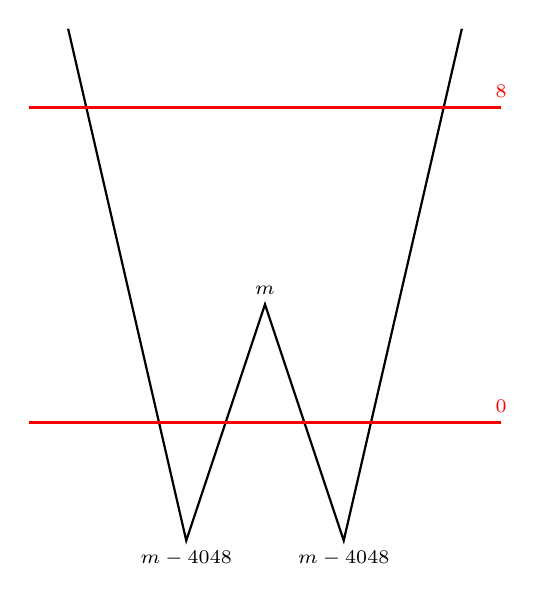
\begin{tikzpicture}[thick,font=\scriptsize,scale=0.5]
				\draw (-5,10)--(-2,-3)node[below]{$m-4048$}--(0,3)node[above]{$m$}--(2,-3)node[below]{$m-4048$}--(5,10);
				\draw[red] (-6,0)--(6,0)node[above]{$0$} (-6,8)--(6,8)node[above]{$8$};
			\end{tikzpicture}
		\end{center}
		Để hàm số có đúng $9$ điểm cực trị $\Leftrightarrow \heva{&m-4048 <0\\&m>0 \\&m \leq 8} \Leftrightarrow 0<m\leq 8$.\\
		Do $m\in\mathbb{Z}$ có $8$ giá trị nguyên của $m$ thỏa đề là $m \in \{1;2;\ldots;8\}$.
	}
\end{ex}

%Câu 44 (TN)
\begin{ex}%%[2D1H2-1]
	Cho $F(x)$ là một nguyên hàm của hàm số $f(x)=\mathrm{e}^{x^2-2x} \left( x^3-2024x \right)$. Hàm số $F(x)$ có bao nhiêu điểm cực trị?
	\choice
	{$2$}
	{\True $3$}
	{$1$}
	{$4$}
	\loigiai{
		Ta có $F' (x) = f(x) = \mathrm{e}^{x^2-2x} \left( x^3-2024x \right)$. \\
		Phương trình $F'(x) =0 \Leftrightarrow x^3-2024x =0 \Leftrightarrow \hoac{& x=0 \\ & x = \sqrt{2\,024} \\ & x = - \sqrt{2\,024}.}$ \\
		Phương trình $F'(x)=0$ có đúng $3$ nghiệm bội lẻ nên hàm số $F(x)$ có $3$ điểm cực trị. 
	}
\end{ex}

%Câu 45 (TN)
\begin{ex}[BỎ]%[2H5N1-2]
	Cho hình trụ có chiều cao bằng $6a$. Biết rằng khi cắt hình trụ đã cho bởi một mặt phẳng song song với trục và cách trục một khoảng bằng $3a$, thiết diện thu được là một hình vuông. Thể tích của khối trụ được giới hạn bởi hình trụ đã cho bằng
	\choice
	{$216\pi a^3$}
	{$150\pi a^3$}
	{$36\pi a^3$}
	{\True $108\pi a^3$}
	\loigiai{
		\begin{center}
			\begin{tikzpicture}[font=\footnotesize, line join=round, line cap=round, >=stealth, scale=0.8] 
				\coordinate (O) at (-2, 3);
				\coordinate (A) at (-4, 3);
				\draw[](0, 3) arc (0:360:2 and 1);
				\draw[dashed] (0, 0) arc (0:180:2 and 1);
				\draw(-4, 0) arc (180:360:2 and 1);
				\draw (-4, 0)--(-4, 3) (0, 0)--(0, 3);
				\filldraw (-2, 0) circle(1pt); \filldraw (-2, 3) circle(1pt); \coordinate (M) at ($(-4, 3)!0.5!(-1, 2.1)$);
				\draw[dashed] (-1,-0.89)--(-4, 0) (-2, 3)--(-2, 0);
				\draw(-4, 3)--(-1, 2.12)--(-1,-0.89);
				\draw(-2.5, 2.56)--(-2, 3) (-2, 3)--(-4, 3);
				\node[right] at (-2, 3) {$O$};
				\node[above left] at (-4, 3) {$A$};
				\node[right] at (-2, 0) {$O'$};
				\node[above] at (-1, 2.1) {$B$};
				\node[right] at (-1,-1.1) {$C$};
				\node[above left] at (-4,-0.9) {$D$};
				\fill (M) circle(1pt) node[shift=(-80:0.25)]{$M$}; 
				\pic[draw, angle radius=2mm, angle eccentricity=2] {right angle=A--M--O};			
			\end{tikzpicture}
		\end{center}
		Theo giả thiết, ta có $OO'=6a$, $OM=3a$. \\
		Do $ABCD$ là hình vuông nên $AB=BC=CD=DA=OO'=6a$. \\
		Xét $\triangle OMA$ vuông tại $M$, ta có $OA=\sqrt{OM^2+MA^2}=\sqrt{9a^2+9a^2}=3\sqrt{2} a$. \\
		Vậy thể tích của khối trụ là $V=\pi \cdot OA^2\cdot OO'=\pi \cdot 18a^2\cdot 6a=108\pi a^3$.}
\end{ex}

%Câu 46 (TN)
\begin{ex}%%[2H5V3-2]
	
	Trong không gian $Oxyz$, cho các điểm $A(0;2;0)$, $B(2;0; 0)$, $C(0; 0;-1)$. Gọi $(S)$ là mặt cầu đi qua bốn điểm $A$, $B$, $C$ và $O$. Tính bán kính $R$ của mặt cầu $(S)$.
	\choice
	{$R=2$}
	{$R=1$}
	{\True $R=\dfrac{3}{2}$}
	{$R=3$}
	\loigiai{
		Gọi phương trình mặt cầu $(S)$ là $x^2+y^2+z^2-2a x-2b y-2c z+d=0$. \\
		Theo giả thiết, ta có $\heva{& A\in (S) \\ & B\in (S) \\ & C\in (S) \\& O\in (S)} \Leftrightarrow \heva{& 4-4b+d=0\\ & 4-4a+d=0\\ & 1+2c+d=0\\ & d=0} \Leftrightarrow \heva{& b=1\\ & a=1\\ & c=-\dfrac{1}{2} \\ & d=0.}$ \\
		Suy ra phương trình mặt cầu $(S)$ là $x^2+y^2+z^2-2x-2y+z=0$. \\
		Mặt cầu $(S)$ có bán kính là $R=\sqrt{a^2+b^2+c^2-d}=\sqrt{1^2+1^2+\left(-\dfrac{1}{2} \right)^2-0}=\dfrac{3}{2}$.}
\end{ex}

%Câu 47 (TN)
\begin{ex}%[2D1V1-2]
	Cho hàm số $y=f(x)$ xác định trên $\mathbb{R}$ và có bảng biến thiên như hình vẽ.
	\begin{center}
		
\begin{tikzpicture}
			\tkzTabInit[nocadre=true, lgt=1.2, espcl=3, deltacl=0.5]
			{$x$ / 0.7,$f'(x)$ /.7,$f(x)$/2} 
			{$-\infty$,$1$,$3$,$+\infty$}
			\tkzTabLine{,+,$0$,-,$0$,+,}
			\tkzTabVar{-/$-\infty$,+/$1$,-/$-3$,+/$+\infty$}
		\end{tikzpicture}
	\end{center}
	Hàm số $y=f(3+x)$ nghịch biến trên khoảng nào dưới đây?
	\choice
	{$(4;6)$}
	{$(-5;3)$}
	{$(1;3)$}
	{\True $(-2;0)$}
	\loigiai{
		Ta có $y'=f'(x+3)$.\\
		Phương trình $y'=0 \Leftrightarrow f'(x+3)=0 \Leftrightarrow \hoac{&x+3=1\\&x+3=3} \Leftrightarrow \hoac{&x=-2\\&x=0.}$\\
		Bảng biến thiên của hàm số $y=f(x+3)$
		\begin{center}
			
\begin{tikzpicture}
				\tkzTabInit[nocadre=true, lgt=1 , espcl=3, deltacl=0.5]
				{$x$ / 0.7,$y'$ /.7,$y$/2}
				{$-\infty$,$-2$,$0$,$+\infty$}
				\tkzTabLine{,+,$0$,-,$0$,+,}
				\tkzTabVar{-/$-\infty$,+/$1$,-/$-3$,+/$+\infty$} 
			\end{tikzpicture}
		\end{center}
		Vậy hàm số $y=f(3+x)$ nghịch biến trên khoảng $(-2;0)$.
	}
\end{ex}

%Câu 48 (TN)
\begin{ex}%%[2H5C1-3]
	Trong không gian $Oxyz$, biết mặt phẳng $(P)$ đi qua điểm $M(1; 2; 3)$ và cắt các trục $Ox$, $Oy$, $Oz$ lần lượt tại ba điểm $A$, $B$, $C$ khác với gốc tọa độ $O$ sao cho biểu thức $\dfrac{1}{OA^2}+\dfrac{1}{OB^2}+\dfrac{1}{OC^2}$ có giá trị nhỏ nhất. Khi đó, mặt phẳng $(P)$ đi qua điểm nào sau đây?
	\choice
	{$(1; 2; 7)$}
	{$(7; 1; 2)$}
	{\True $(7; 2; 1)$}
	{$(2; 7; 1)$}
	\loigiai{
		Gọi $A(a;0;0)$, $B(0;b;0)$ và $C(0;0;c)$ lần lượt là giao điểm của mặt phẳng $(P)$ với các trục $Ox$, $Oy$ và $Oz$.\\
		Phương trình theo đoạn chắn của mặt phẳng $(P)$ là $\dfrac{x}{a}+\dfrac{y}{b}+\dfrac{z}{c}=1$.\\
		Mà $M\in (P)$ nên $\dfrac{1}{a}+\dfrac{2}{b}+\dfrac{3}{c}=1$.\\
		Áp dụng bất đẳng thức Cauchy-Schwarz, ta có
		\allowdisplaybreaks \begin{eqnarray*}
			1=\left(1\cdot \dfrac{1}{a}+2\cdot \dfrac{1}{b}+3\cdot \dfrac{1}{c}\right)^2&\leq& \left(1^2+2^2+3^2\right)\left(\dfrac{1}{OA^2}+\dfrac{1}{OB^2}+\dfrac{1}{OC^2}\right)\\
			&=& 14\cdot\left(\dfrac{1}{OA^2}+\dfrac{1}{OB^2}+\dfrac{1}{OC^2}\right).
		\end{eqnarray*}
		Suy ra $\dfrac{1}{OA^2}+\dfrac{1}{OB^2}+\dfrac{1}{OC^2}\geq \dfrac{1}{14}$.\\
		Dấu \lq\lq $=$\rq\rq~ xảy ra khi và chỉ khi  $\heva{&a=2b=3c\\&\dfrac{1}{a}+\dfrac{2}{b}+\dfrac{3}{c}=1}\Leftrightarrow\heva{&b=\dfrac{a}{2}\\&c=\dfrac{a}{3}\\&\dfrac{1}{a}+\dfrac{4}{a}+\dfrac{9}{a}=1}\Leftrightarrow \heva{&a=14\\&b=7\\&c=\dfrac{14}{3}.}$\\
		Suy ra phương trình mặt phẳng $(P)$ là $\dfrac{x}{14}+\dfrac{y}{7}+\dfrac{3z}{14}=1$.\\
		Vậy mặt phẳng $(P)$ đi qua điểm có tọa độ $(7;2;1)$.
	}
\end{ex}

%Câu 49 (TN)
\begin{ex}[BỎ]
	Cho hàm số $f(x)$ có đạo hàm liên tục trên $\mathbb{R}$, thỏa mãn $f(2)=5$ và $\displaystyle\int\limits_0^2f(x)\mathrm{\,d} x=8$. Tính tích phân $I=\displaystyle\int\limits_0^2 x f'(x)\mathrm{\,d}x$.
	\choice
	{$I=-2$}
	{\True $I=2$}
	{$I=0$}
	{$I=-3$}
	\loigiai{
		Đặt $\heva{&u=x\\&\mathrm{d}v=f'(x)\mathrm{\,d}x}\Rightarrow\heva{&\mathrm{d}u=\mathrm{\,d}x\\&v=f(x).}$\\
		Khi đó $I=xf(x)\Big|_0^2-\displaystyle\int\limits_0^2f(x)\mathrm{\,d}x=2f(2)-0f(0)-8=2\cdot 5-8=2$.
	}
\end{ex}

%Câu 50 (TN)
\begin{ex}%%[1D6C2-3]
	Cho các số thực dương $a$, $b$, $c$ (với $a$, $c$ khác $1$) thỏa mãn các điều kiện \break$\log_a \left(a^4c\right)=\log_c\left(bc^2\right)$ và $2\log_ac+\log_cb=8$. Tính giá trị của biểu thức $P=\log_ab-\log_c\left(ab^2\right)$.
	\choice
	{\True $P=-\dfrac{1}{2}$}
	{$P=-2$}
	{$P=-\dfrac{3}{2}$}
	{$P=\dfrac{3}{2}$}
	\loigiai{
		Ta có 
		\allowdisplaybreaks \begin{eqnarray*}
			\log_a\left(a^4c\right)=\log_c \left(bc^2\right)&\Leftrightarrow&\log_aa^4+\log_ac=\log_cb+\log_cc^2\\
			&\Leftrightarrow&4+\log_ac=\log_cb+2\\
			&\Leftrightarrow&\log_ac-\log_cb=-2.
		\end{eqnarray*}
		Khi đó, ta có hệ phương trình $\heva{&\log_ac-\log_cb=-2\\&2\log_ac+\log_cb=8}\Leftrightarrow\heva{&\log_ac=2\\&\log_cb=4.}$\\
		Do đó
		\allowdisplaybreaks \begin{eqnarray*}
			P&=&\log_ab-\log_c\left(ab^2\right)\\
			&=&\log_ac\cdot\log_cb-\log_ca-\log_cb^2\\
			&=&\log_ac\cdot\log_cb-\dfrac{1}{\log_ac}-2\log_cb\\
			&=&2\cdot 4-\dfrac{1}{2}-2\cdot 4=-\dfrac{1}{2}.
		\end{eqnarray*}
	}
\end{ex}
\Closesolutionfile{ans}
\Closesolutionfile{ansbook}

\begin{indapan}
	{ans/ans\currfilebase}
\end{indapan}
